\documentclass[border=10pt]{standalone}
\usepackage{tikz}
\usetikzlibrary{shapes.geometric, arrows.meta, positioning, shapes}

\begin{document}

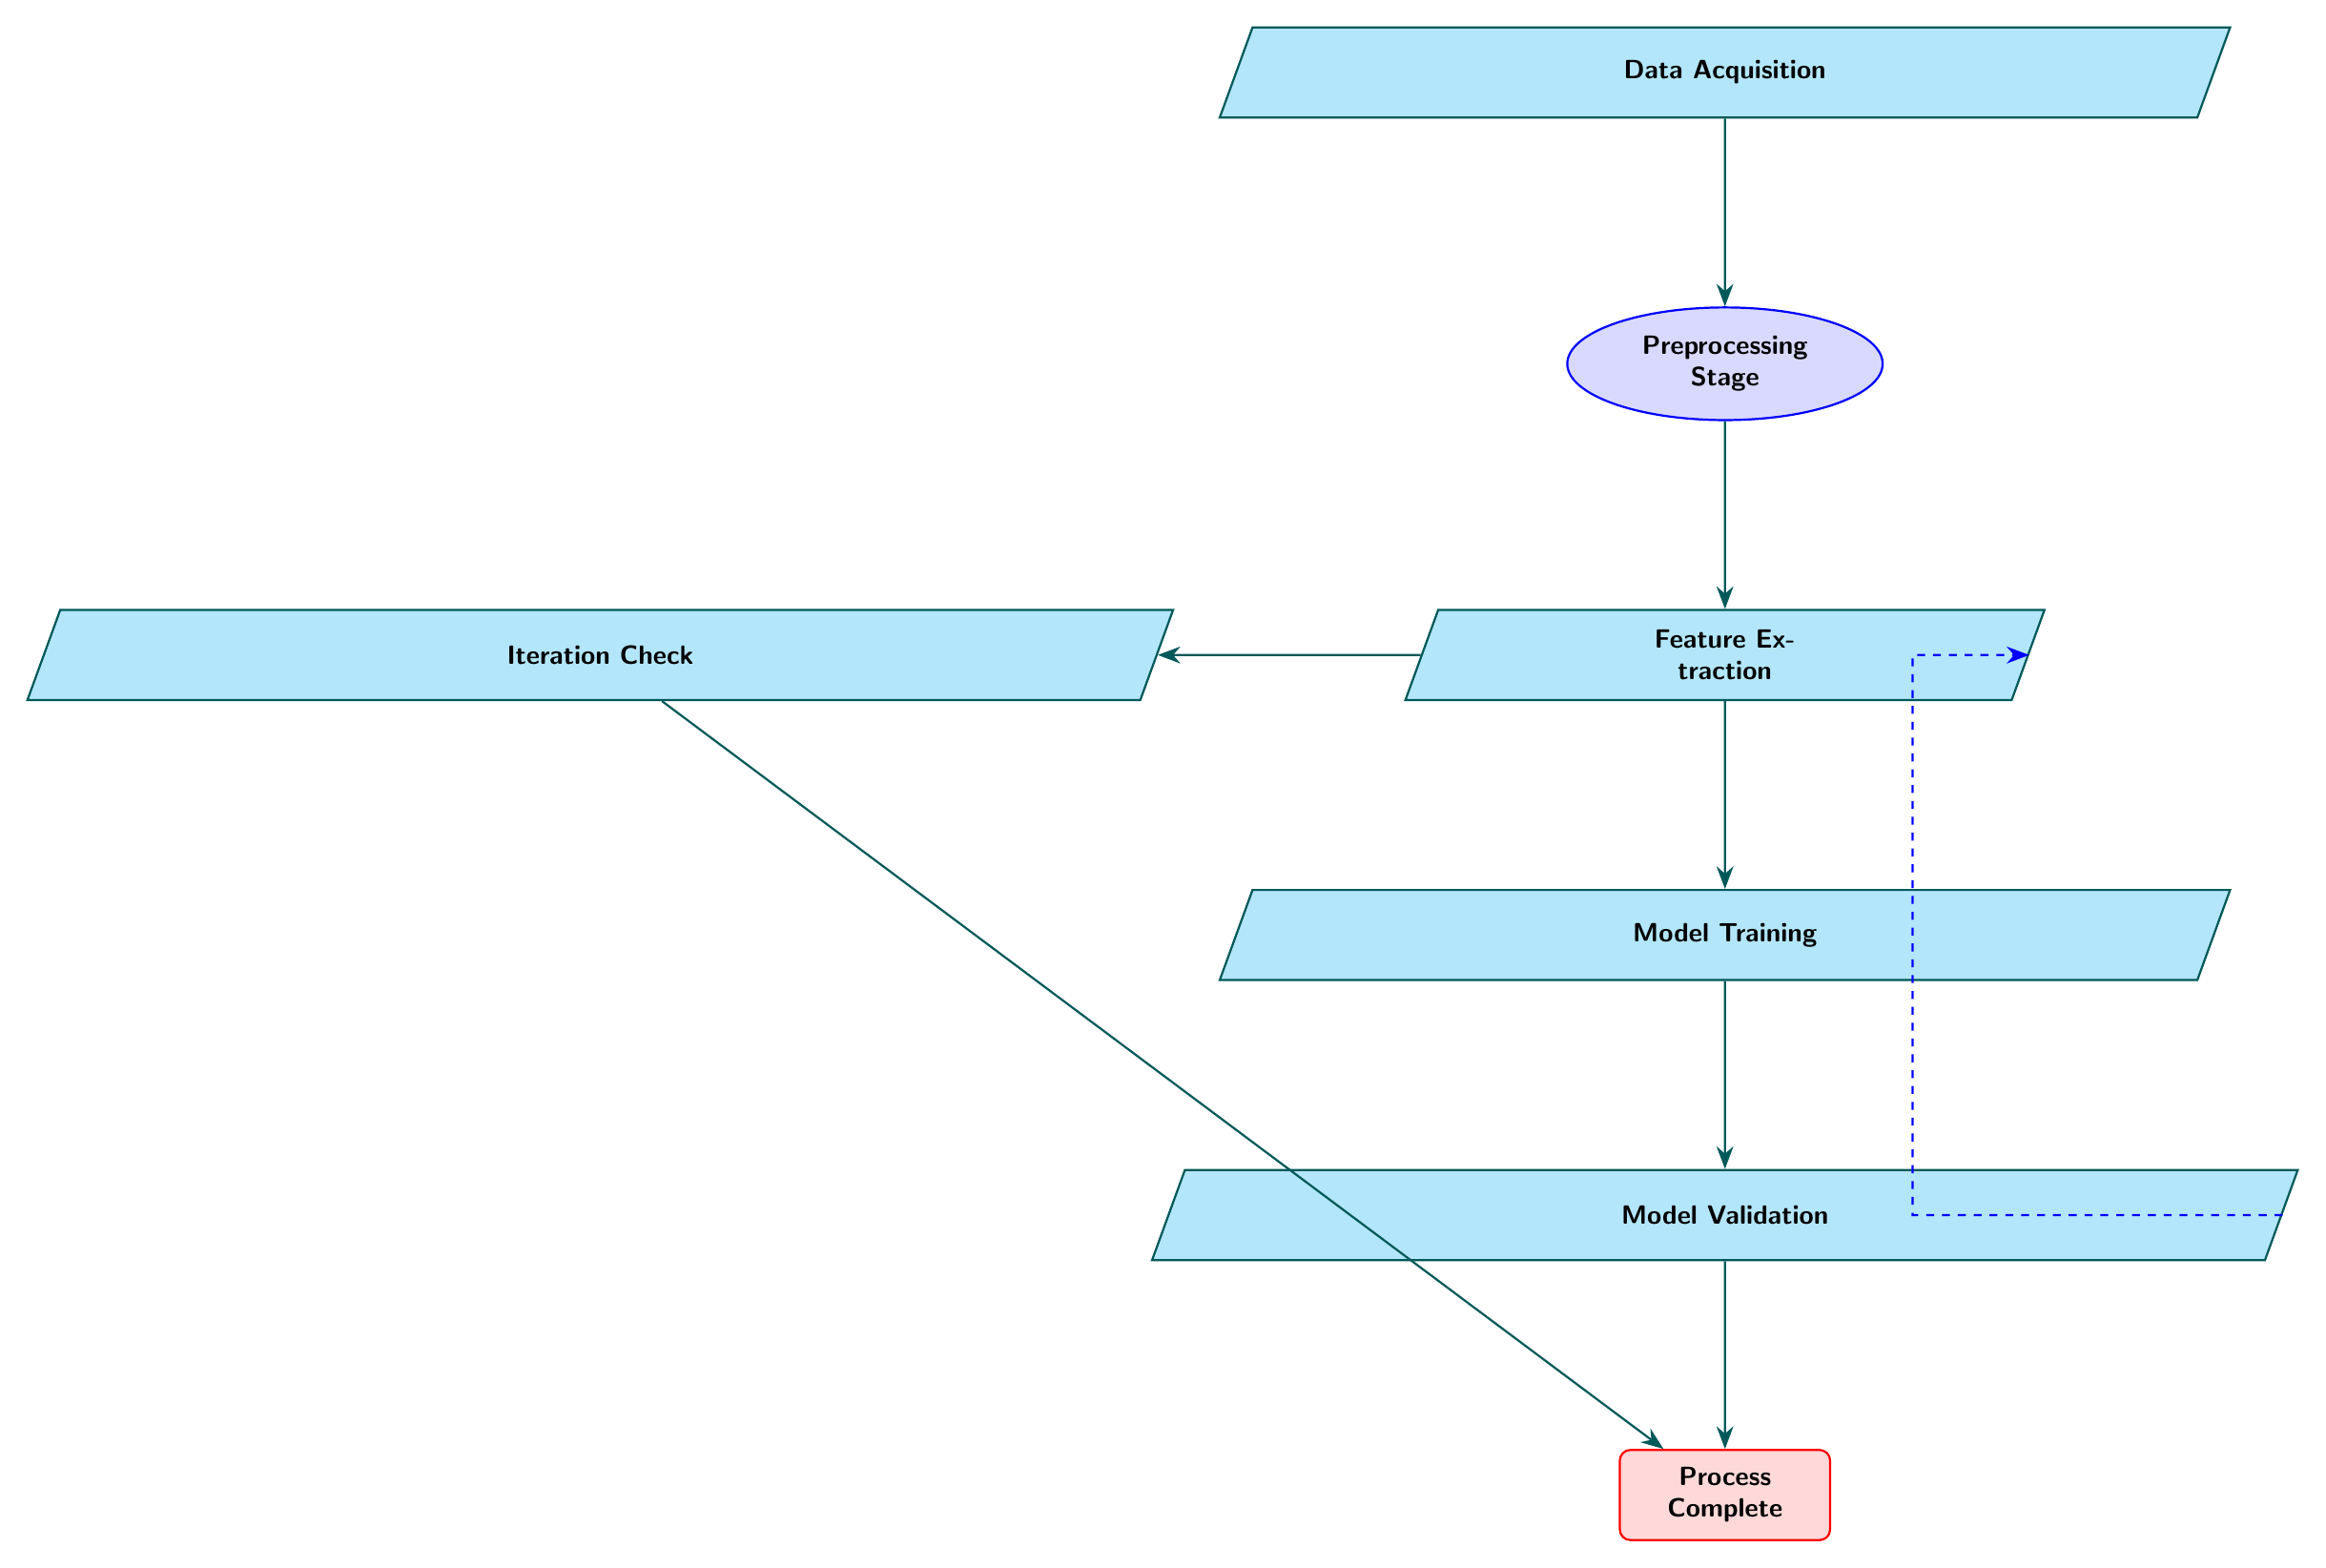
\begin{tikzpicture}[
    node distance = 2.5cm,
    auto,
    parallelogram/.style={trapezium, trapezium left angle=70, trapezium right angle=110, 
                          minimum width=6cm, minimum height=1.2cm, text centered, align=center,
                          draw=teal!70!black, fill=cyan!30, thick, text width=5.5cm,
                          font=\sffamily\bfseries},
    ellipsenode/.style={ellipse, minimum width=4.2cm, minimum height=1.5cm, 
                        text centered, align=center, draw=blue, fill=blue!15, thick,
                        font=\sffamily\bfseries},
    roundedbox/.style={rectangle, rounded corners, minimum width=2.8cm, 
                       minimum height=1.2cm, text centered, align=center, draw=red, 
                       fill=red!15, thick, font=\sffamily\bfseries},
    arrow/.style={-{Stealth[length=3mm]}, thick, draw=teal!70!black},
    dashedarrow/.style={-{Stealth[length=3mm]}, thick, dashed, blue}
]

% Nodes
\node (acquisition) [parallelogram] {Data Acquisition};
\node (preprocessing) [ellipsenode, below=of acquisition] {Preprocessing\\Stage};
\node (feature) [parallelogram, below=of preprocessing] {Feature Ex-\\traction};
\node (training) [parallelogram, below=of feature] {Model Training};
\node (validation) [parallelogram, below=of training] {Model Validation};
\node (complete) [roundedbox, below=of validation] {Process\\Complete};
\node (iteration) [parallelogram, left=3.5cm of feature] {Iteration Check};

% Arrows
\draw [arrow] (acquisition) -- (preprocessing);
\draw [arrow] (preprocessing) -- (feature);
\draw [arrow] (feature) -- (training);
\draw [arrow] (training) -- (validation);
\draw [arrow] (validation) -- (complete);
\draw [arrow] (feature) -- (iteration);
\draw [dashedarrow] (validation) -- ++(2.5,0) |- (feature);
\draw [arrow] (iteration) -- (complete);

\end{tikzpicture}

\end{document}
